\paragraph{Application} Maximal functions and counterexamples. Q: Given a collection $\C=\{C\}$ of sets, for which class of funcions do we have
\[\lim_{\diam(C)→0,\ c∈\C}\frac1{|C|}∫_Cf(x-y)\md y=f(x)\quad x-\text{a.e.}?\]
Seen:\[(M_\C f)(x)=\sup_{c∈\C}\frac1{|C|}∫_C|f(x)-y)|\md y\]
$\C=\{\text{bals}\}$, weak-type (1,1)inequality for $M_\C⇒$ a.e.\ convergenc of averages. A converse also holds!

$\{\mdμ_j\}_{j=1}^∞$ collection of finite, nonnegative measures on $ℝ^d:\supp(μ_j)⊂K⊂⊂ℝ^d$. Define the maximal operator \[(Mf)(x)=\sup_j|f*μ_j|(x).\]

\begin{pro}$1\leq p<∞$. Assume for each $f∈L^p(ℝ^d)$ that $(Mf)(x)<∞$ for some set of $x$ having positive measure. Then $f↦Mf$ if of wak-type $(p,p)$
	\[∃A<∞:|\{x∈ℝ^d:(Mf)(x)>α\}|\leq\frac A{α^p}\|f\|_{L^p} \quad(∀α>0)\]
\end{pro}

\begin{lem}
	$\{E_j\}$ collection of subsets of a fixed compact set: \[\sum_{j=1}^∞|E_j|=∞.\] Then there exists a sequenc of translates $F_j=E_jx_j$:
	\[\limsup F_j=\bigcap_{k=1}^∞(\bigcup_{j=k}^∞F_j)=ℝ^n\quad\text{(a.e.)}\]
\end{lem}
The above set equals $\{x∈ℝ^d:x∈F_j\text{ infinitely often}\}$.
\[\liminf F_j=\bigcup_{k=1}^∞(\bigcup_{j=k}^∞F_j)\]
is a subset.
\begin{proof}[Proof of Lemma]
	$Q⊂ℝ^d$ unit cube. $A_1,A_2⊂Q$. Then $∃h∈ℝ^d:|A_1∩(A_2-h)|\geq2^{-d}|A_1||A_2|$.
	\begin{figure}[h]
		\centering
		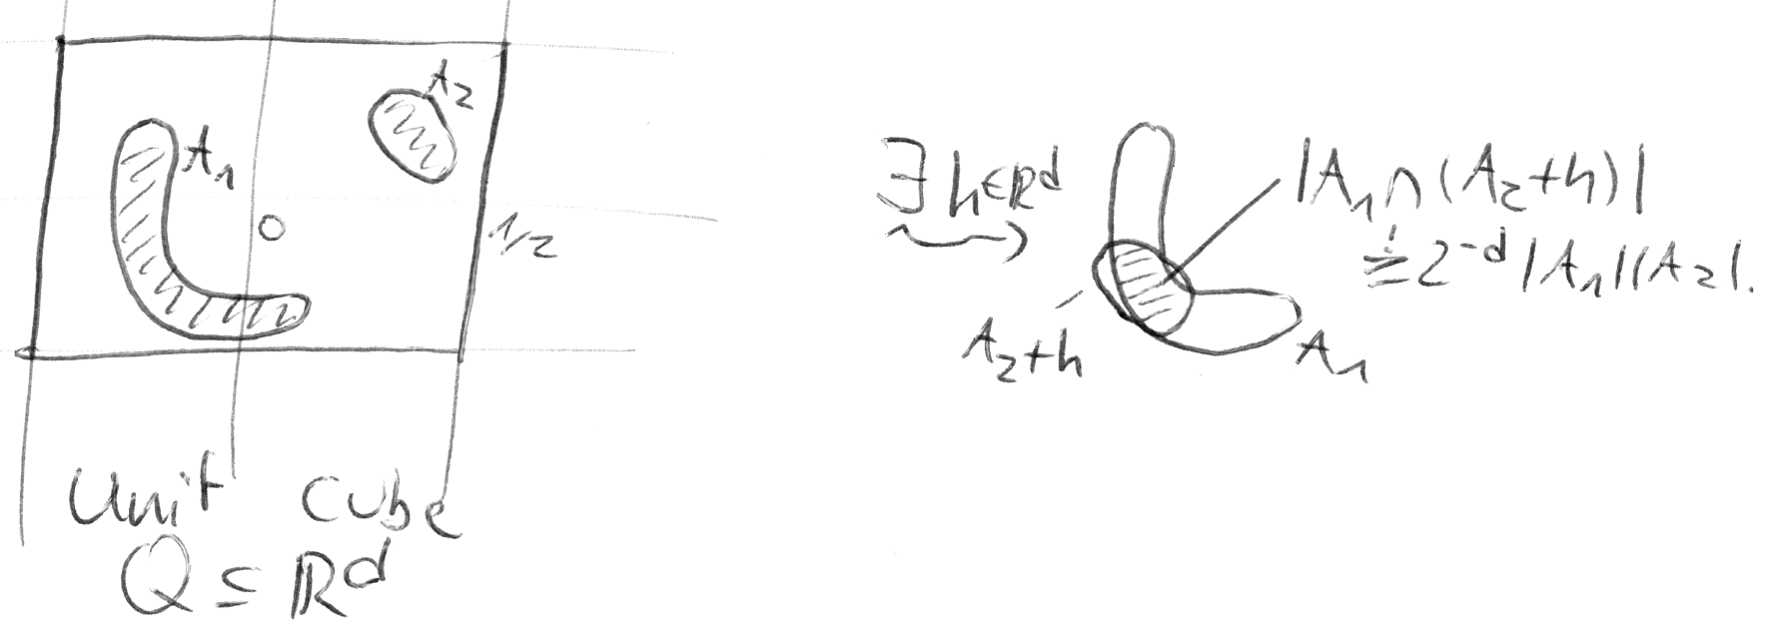
\includegraphics[height=5cm]{lec09_01}
		\caption{Translation of subsets $A_1$ and $A_2$ of a unit cube $Q$.}
	\end{figure}
	Why?
	\[η(x)=ι_{ℝ^d}χ_{A_1}(y)χ_{A_2}(x+y)\md y\simχ_{A_1}*χ_{A_1}(x)\]
	\[∫_{ℝ^d}|A_1||A_1|\]
	\[\supp(η)⊂Q^*\]
	$|Q^*|=2^d$. 
	\[∃h∈Q^*:η(h)\geq\avg_{Q^*}(η)=\frac1{|Q^*|}∫_{ℝ^d}η=\frac{|A_1||A_2|}{2^d}\]
	Wlog $\supp(E_j)⊂Q$.

	Step 2: There exist translates $F_j=E_j+x_j$ that cover $Q$ at least once.
	\[Q⊂\bigcup_j F_j\]
	Why? $F_1=E_1$. Suppose (inductively) that $F_1,…,F_{j-1}$ have been constructed. Let $A_1=Q∩(F_1∪…∪F_{j-1})^\complement$ and $A_2=E_j$. Step 1 $⇒∃h:|A_1∩(A_2-h)|\geq 2^{-d}|A_1||A_2|$. Set $F_j=A_2-h=E_j-h$. Let $p_j=|Q∩(F_1∪…∪F_j)|$. Then \[jvp_j=p_{j-1}+|\underbrace{Q∩(F_1∪…∪F_{j-1})^\complement}_{A_1}∩\underbrace{F_j}_{A_2-h}|=p_{j-1}+|A_1∩(A_2-h)|\geq p_{j-1}+2^{-d}|A_1||E_j|=p_{j-1}+2^{-d}(1-p_{j-1})|E_j|\]
	\[\therefore p_j-p_{j-1}\geq2^{-d}(1-p_{j-1})|E_j|\]
	\[\sum_{j=2}^∞(p_j-p_{j-1})=\lim_{j→∞}p_j-p_1\therefore\lim_jp_j=1\]
	Step 3: Decompose (twice) $\{E_j\}$ into a countable infinite number of subcollections so that on each subcollection the sum of the measures diverges.
\end{proof}
\begin{proof}[Proof of Proposition]
	Take a baoo $B$ sucth that $B\supset Q+K$. $\supp(F)⊂Q⇒\supp(F*⇔_j)⊂⇒\supp(Mf)⊂B$. Key: Estimate (*) (the violation of the weak type estimate) holds if $\supp(f)⊂Q$. For each $k,∃α_k>0∃g_k⊂L^p:\supp(g_k)⊂Q$ such that \[|\{x∈B:Mg_k(x)>α_\}|\geq\frac{2^k}{α_k^p}\|g_k\|_{L^p}^p\]
	Replace $g_k$ by $\tilde g_k=\frac k{α_k}g_k$.
	\[\frac{2^k}{k^p}\leq\frac{|\{x∈B:M\tilde g_k(x)>k\}|}{\|\tilde g_k\|_{L^p}^p}→∞\quad\text{as} k→∞\]
	$\therefore$ Tthere exists a sequence $\{f_k\}⊂L^p$ and a sequence of constans $R_k→∞$ such that (if $E_k=\{x∈B:M f_k(x)>R_k\}$)
	\[\sum_k|E_k|=∞\qquad\sum_k\|f_k\|_{L^p}^p<∞.\]
	\begin{rem} 
		$\mdμ_j\geq 0$ wlog $f_k\geq 0$. 
	\end{rem}
	By the lemma $∃\{x_k\}$ such that $F_k=E_k+x_k$ satisfy $\limsup F_k=ℝ^d$ (a.e). Let
	\[\tilde f_k(x)=f_k(x+x_k),\qquad F(x)=\sup_k\tilde f_k(x)\]
	Then \[M(F)=\sup_j|F*⇔_j|=\sup_j|(\sup_k\tilde f_k)*⇔_j|\geq\sup_k\sup_j|\tilde f_k*μ_j|=\sup_kM(\tilde f_k)\]
	Also $M(\tilde f_k)>R_k$ on $F_k\therefore M(F)=∞$ a.e. Check $f∈L^p$: \[|F|^p=|\sup_k\tilde f_k|^p\leq\sum_p|\tilde f_k|^p\]
	\[\|F\|_{L^p}^p\leq\sum_k\|f_ku|_{L^p}^p<∞\]
	Full conclusion
	\[f=\sum fχ_{Q_j}=:\sum f_j\]
	\[M(f)\leq\sum_jM(f_j)\]
\end{proof}

\begin{exa}%1
	Rectangles with arbitrary orientation
	\[\C=\R=\{\text{\highl{all} retangles in $ℝ^2$ centered at $0$}\}\]
	\begin{figure}[H]
		\centering
		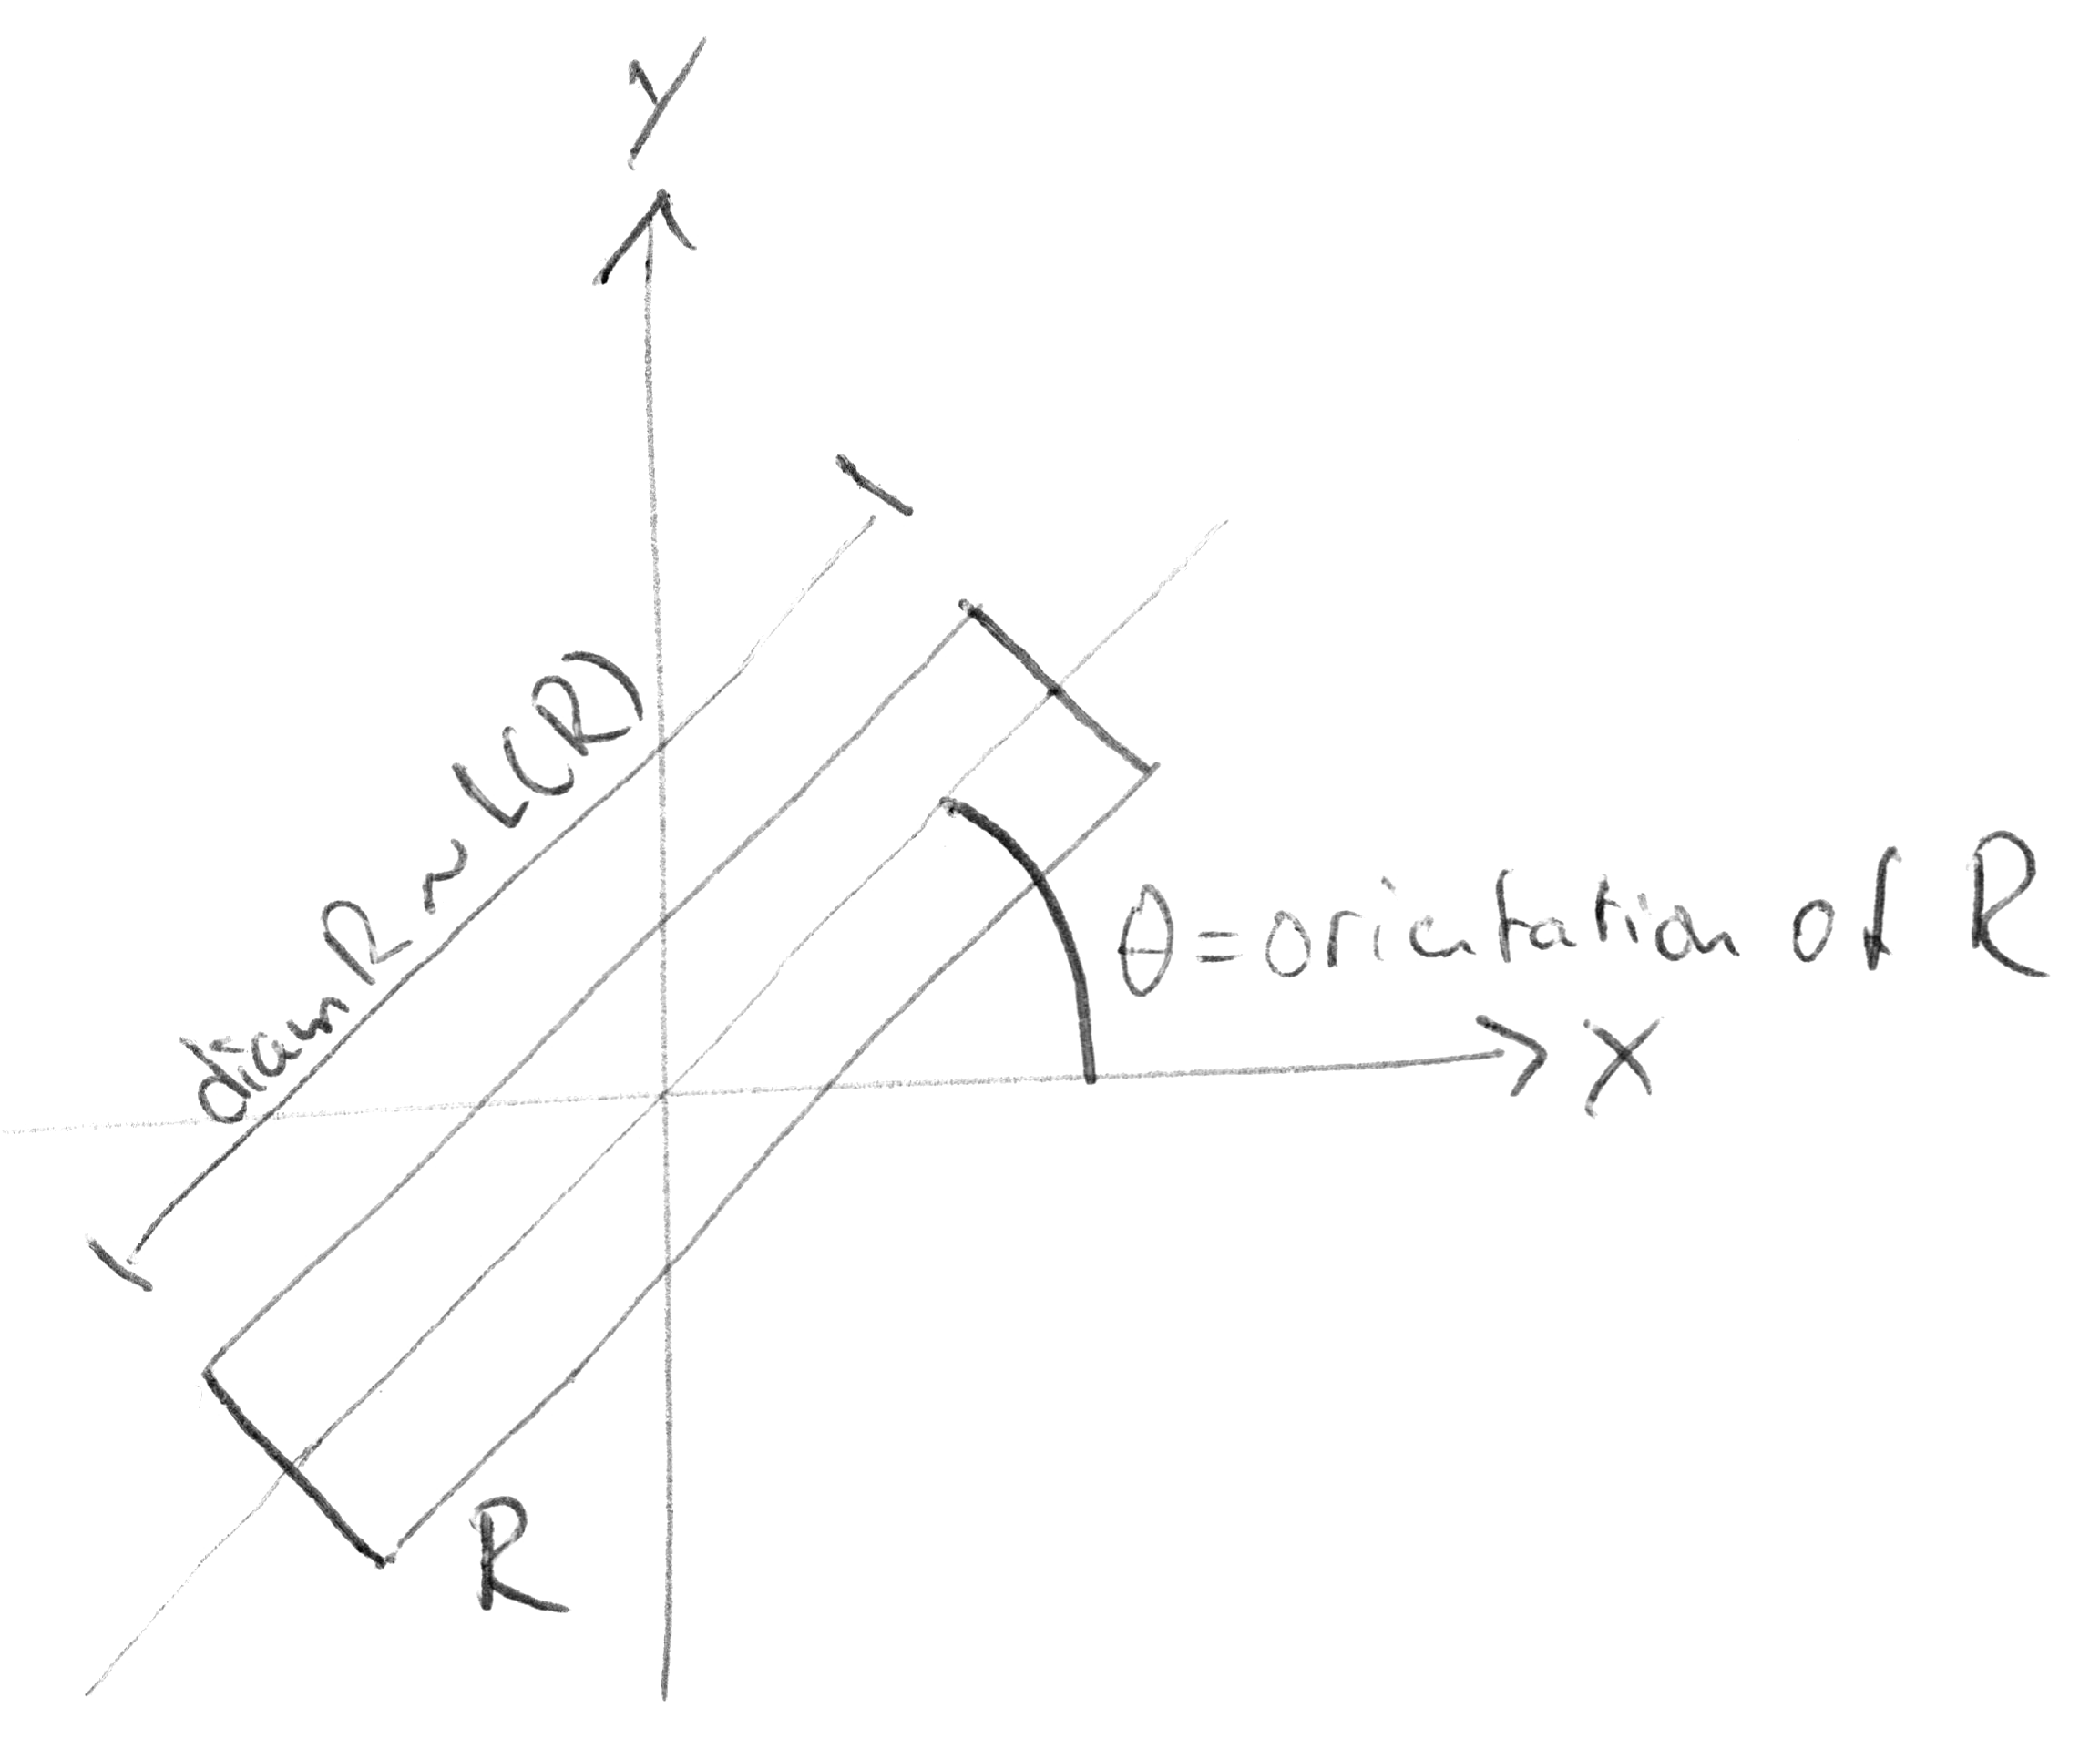
\includegraphics[height=7cm]{lec09_02}
	\end{figure}
\end{exa}
\begin{cor}
	Given $1\leq p<∞,∃f∈L^p(ℝ^)$ such that \[\limsup_{\diam(R)→0R∈\R}\frac1{|R|}∫_Rf(x-y)\md y=∞\quad (x-\text{a.e.})\]
\end{cor}
Idea: Use the $ε$-Kakeya set to show that $M$ is not weak $(p,p)$
\[(Mf)(x)=\sup_{\diam(R)<8}\frac1{|R|}|∫_Rf(x-y)\md y|\]
Let $E=\bigcup_{j=1}^{2^N}R_j$ as before. $\|χ_E\|_{L^p}^p=|E|<ε$. If $x∈\tilde R_j$, then $∃$ rectangle $R$ such that
\begin{itemize}
	\item $R$ is centered at $x$
	\item $\diam(R)\leq 8$
	\item $|R∩R_j|\geq\frac1{12}|R|$
\end{itemize}
\begin{figure}[H]
	\centering
	\subfigure{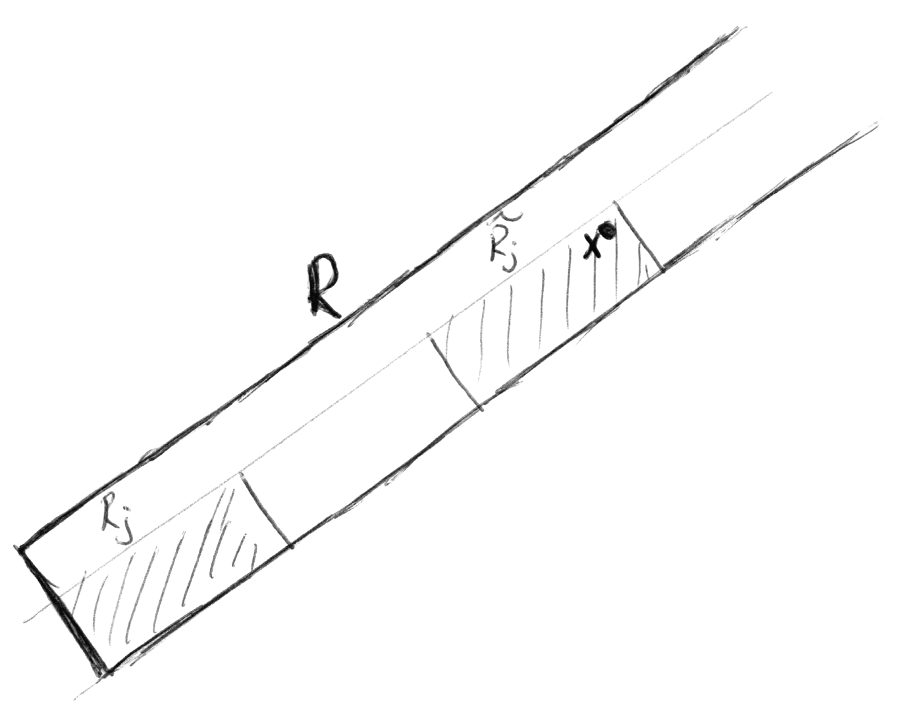
\includegraphics[height=4cm]{lec09_03}}\\
	\subfigure{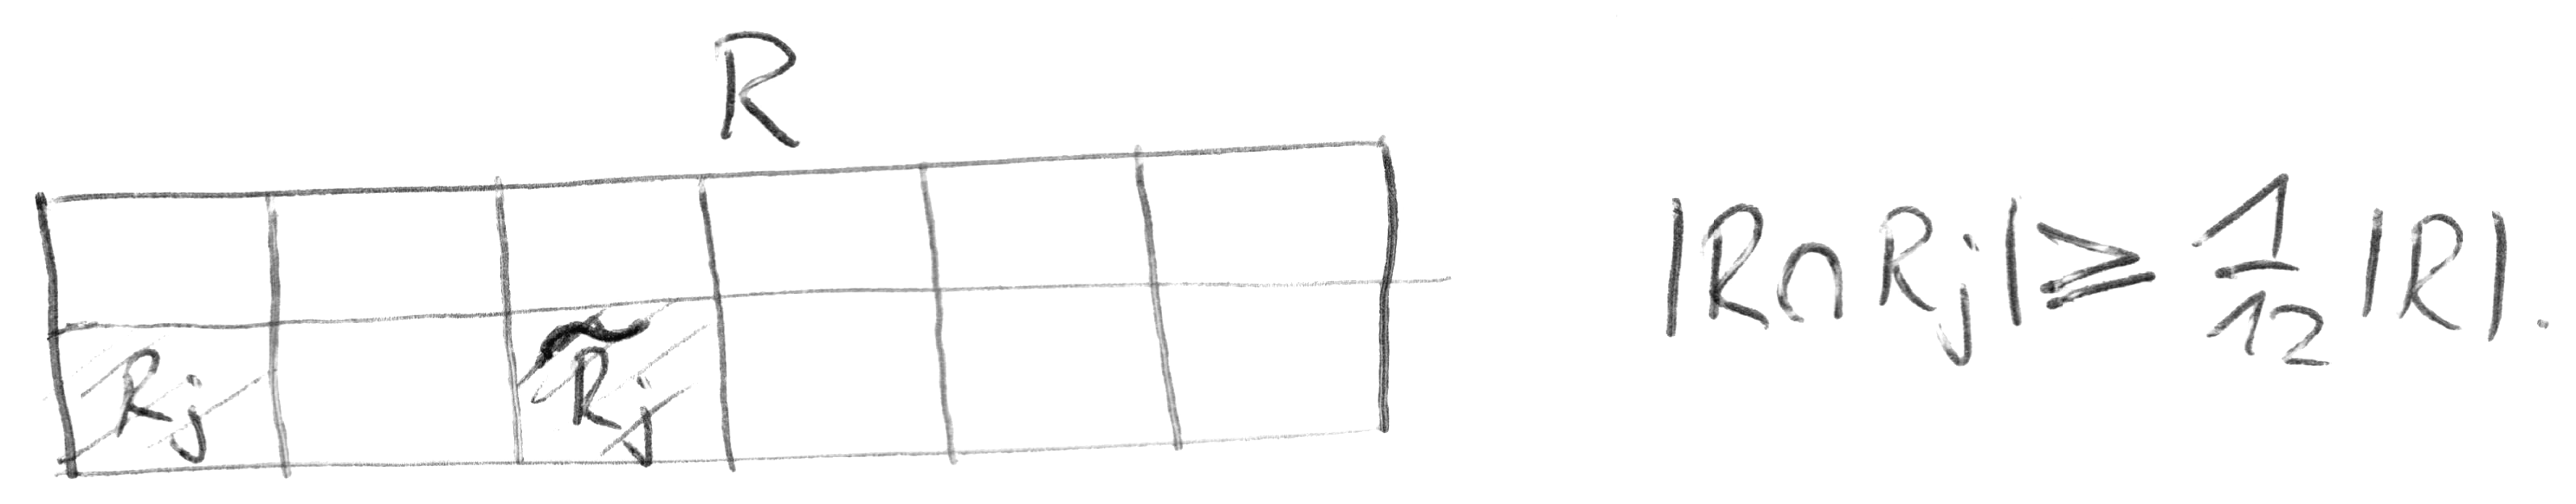
\includegraphics[height=1.5cm]{lec09_04}}
\end{figure}
$y∈x-E=-(E-x),\ y-x∈-E,\ x-y∈ E$
\[M(χ_E)(x)\geq\dashint_{R-x}χ_E(x-y)\md y=\frac{|(R-x)∩(E-x)}{|R|}\geq\frac1{12}\]

Conclusion: $Mχ_E\geq\frac1{12}$ on the set $\bigcup_{j-1}^{2^N}\tilde R_j$ (of measure 1)
\[∀A>0∃\text{set}E|\{x∈ℝ^d:Mχ_E>α\}|\leq Aα^{-p}\|χ_E\|_{L]p}^p\]
does not hold! $\therefore M$ is not of weak typ $(p,p)$.

Note, that this is not the complete proof. Therefore still have to replace 8 by $δ$.
